\subsection{Method}

The ANN part required at least one simple ANN model and one more
advanced ANN architecture \cite{assignment5sc28}. Therefore, three
models were compared: a feedforward NARX ANN, a GRU, and an LSTM.

Since the system is dynamic, past inputs and outputs are needed. A
nonlinear autoregressive model with exogenous input (NARX) is written as

\begin{equation}
\begin{aligned}
\hat{\theta}(k)
=
f\big(&
\theta(k-1),\ldots,\theta(k-n_a),\\
&
u(k-1),\ldots,u(k-n_b)
\big),
\end{aligned}
\label{eq:ann_narx_general}
\end{equation}

where \(n_a\) and \(n_b\) are the output and input memory lengths. The
simple ANN approximates \(f(\cdot)\) with a feedforward network with one
hidden layer of 50 neurons, following the practical-session structure
\cite{course5sc28}. Both memory lengths were set to 15.
In prediction mode, the delayed angles in \eqref{eq:ann_narx_general}
are measured values. In simulation mode, the model must use its own
previous outputs instead of the measured previous angles. In other
words, simulation uses the same model structure as
\eqref{eq:ann_narx_general}, but replaces the measured delayed angles
\(\theta\) by the simulated delayed angles
\(\hat{\theta}_{\mathrm{sim}}\). This is why simulation is a stricter
test than one-step prediction: small errors can be fed back into the
model and affect later samples.

The GRU and LSTM use the same history length \(H=15\), but read it as an
ordered sequence of voltage-angle pairs instead of one flattened vector.
A recurrent network updates an internal state while reading this
sequence:

\begin{equation}
\begin{aligned}
\mathbf{h}_j
&=
g_{\mathrm{RNN}}(\mathbf{h}_{j-1}, [u(j),\theta(j)]),\\
\hat{\theta}(k)
&=
W_o\mathbf{h}_{k-1}+b_o .
\end{aligned}
\label{eq:ann_recurrent_state}
\end{equation}

The hidden state \(\mathbf{h}_j\) stores information from previous
samples. The GRU is simpler, while the LSTM has a more detailed memory
mechanism \cite{course5sc28,cho2014gru,hochreiter1997lstm}.
All models were trained using normalized data, mean squared error loss,
and the Adam optimizer \cite{kingma2014adam}. The known data were split
into 70\% training, 15\% validation, and 15\% test data. The complete
identification dataset contained 35000 measured samples, giving 24500
raw training samples, 5250 validation samples, and 5250 test samples.
Because the ANN inputs use past samples, the supervised training set was
slightly smaller: 24485 training examples for history length 15.

Seven ANN configurations were compared: one NARX ANN, one GRU, one final
LSTM, and four LSTM tuning runs. The LSTM tuning runs are shown in
Table~\ref{tab:lstm_tuning}.

\begin{table}[htbp]
\caption{LSTM tuning results on the held-out test split.}
\centering
\begin{tabular}{cccc}
\toprule
History & Hidden size & Prediction RMSE & Simulation RMSE \\
\midrule
10 & 20 & 0.458 deg & 2.433 deg \\
15 & 20 & 0.394 deg & 2.227 deg \\
15 & 40 & 0.267 deg & 2.384 deg \\
15 & 60 & 0.218 deg & 1.771 deg \\
\bottomrule
\end{tabular}
\label{tab:lstm_tuning}
\end{table}

History length 15 and hidden size 60 gave the best LSTM simulation
result. This architecture was then retrained with the NARX and GRU for
the final comparison. Since training is stochastic, the retrained LSTM
result in Table~\ref{tab:ann_results} differs slightly from the tuning
value.

\subsection{ANN Results}

Table~\ref{tab:ann_results} compares the simple NARX ANN, GRU, and
LSTM. The project files report errors in radians and degrees; the table
uses degrees for readability.

\begin{table}[htbp]
\caption{ANN results on the held-out test split.}
\centering
\begin{tabular}{lcc}
\toprule
Model & Prediction RMSE & Simulation RMSE \\
\midrule
Simple NARX ANN & 2.442 deg & 16.130 deg \\
Advanced GRU ANN & 0.202 deg & 2.031 deg \\
Advanced LSTM ANN & 0.235 deg & 1.893 deg \\
\bottomrule
\end{tabular}
\label{tab:ann_results}
\end{table}

Fig.~\ref{fig:ann_errors} shows the same comparison. The left plot uses a
logarithmic scale because the NARX simulation error is much larger; the
right plot zooms in on GRU and LSTM.

\begin{figure}[htbp]
\centerline{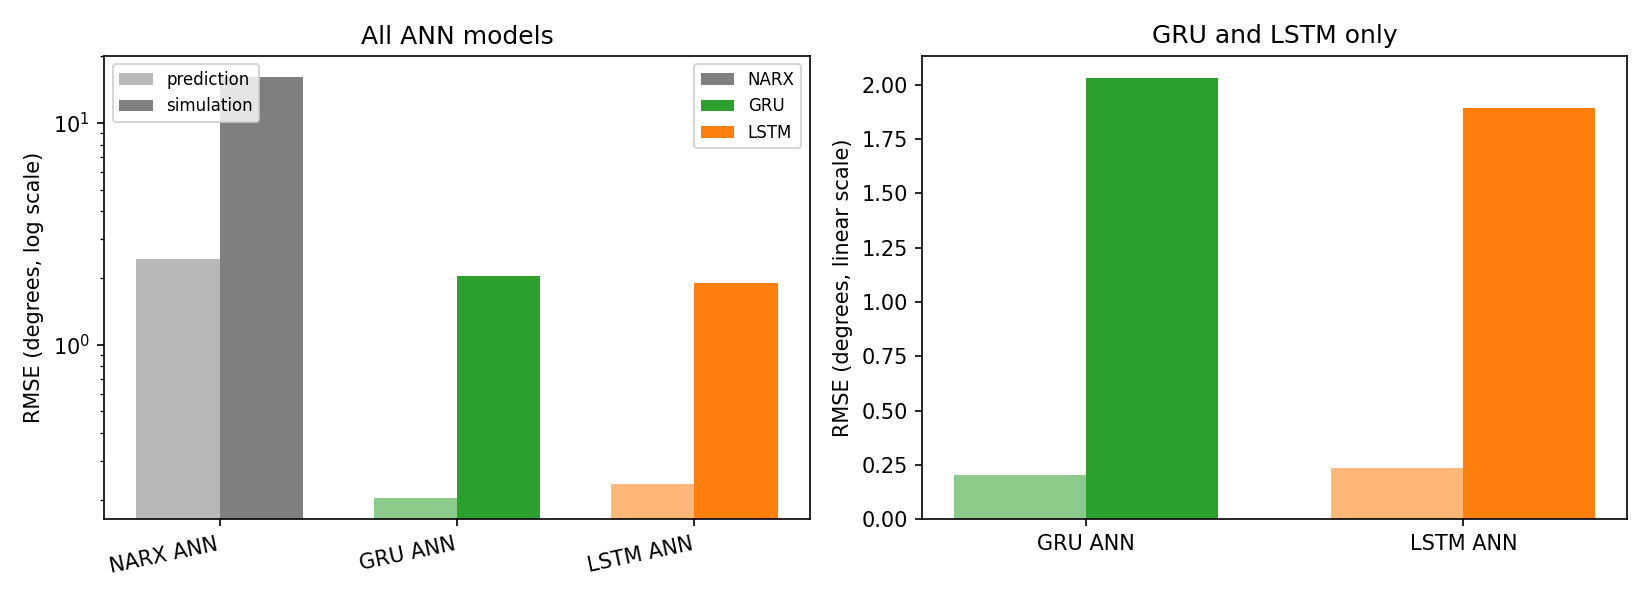
\includegraphics[width=\columnwidth]{figures/ann_three_model_comparison.png}}
\caption{Prediction and simulation RMSE for the three ANN models.}
\label{fig:ann_errors}
\end{figure}

Both recurrent models clearly outperformed the simple NARX ANN. The GRU
gave the best prediction result, while the LSTM gave the best simulation
result. This is reasonable because prediction uses measured past angles,
whereas simulation feeds the model's own predictions back into the
input.

Fig.~\ref{fig:ann_prediction} shows the prediction errors for the recurrent models.
This plot is used instead of only showing angle trajectories, because
the GRU and LSTM trajectories are very close to the measured angle.

\begin{figure}[htbp]
\centerline{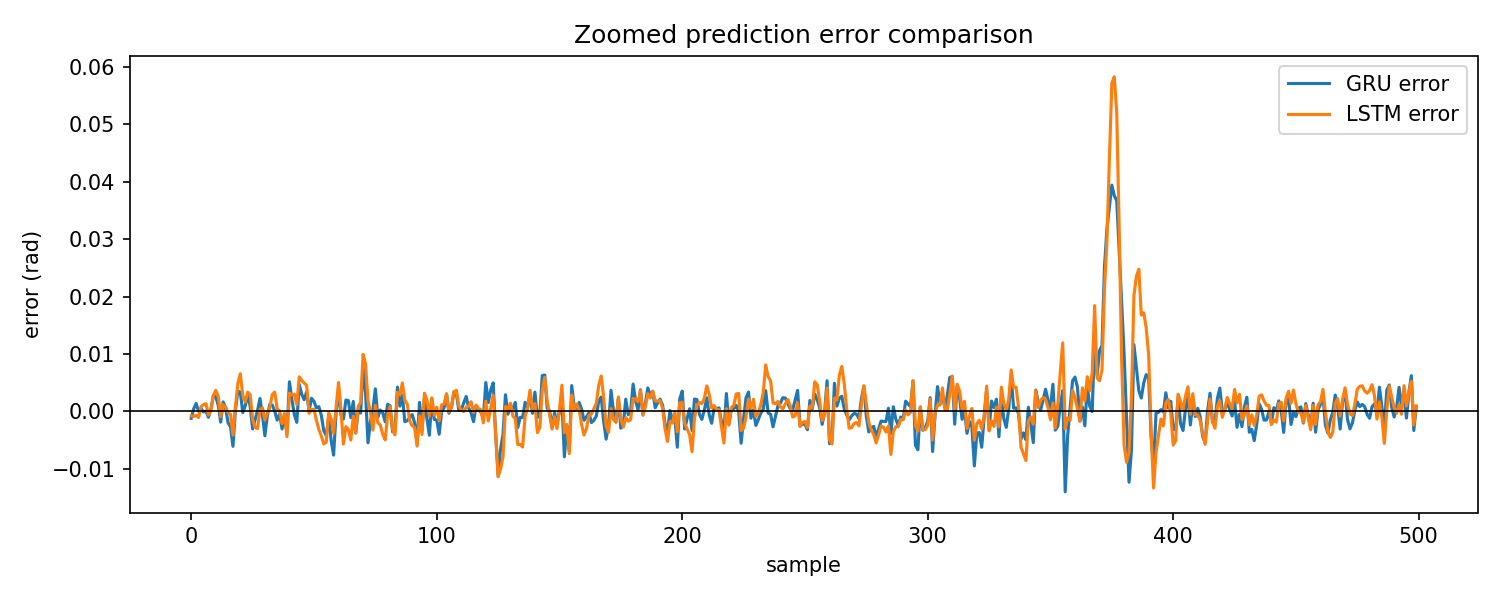
\includegraphics[width=\columnwidth]{figures/ann_prediction_error_zoom.png}}
\caption{Prediction error for the GRU and LSTM models.}
\label{fig:ann_prediction}
\end{figure}

Fig.~\ref{fig:ann_simulation} shows the simulation errors for the recurrent models.
This is the more important long-term comparison, because the model must
feed back its own previous predictions.

\begin{figure}[htbp]
\centerline{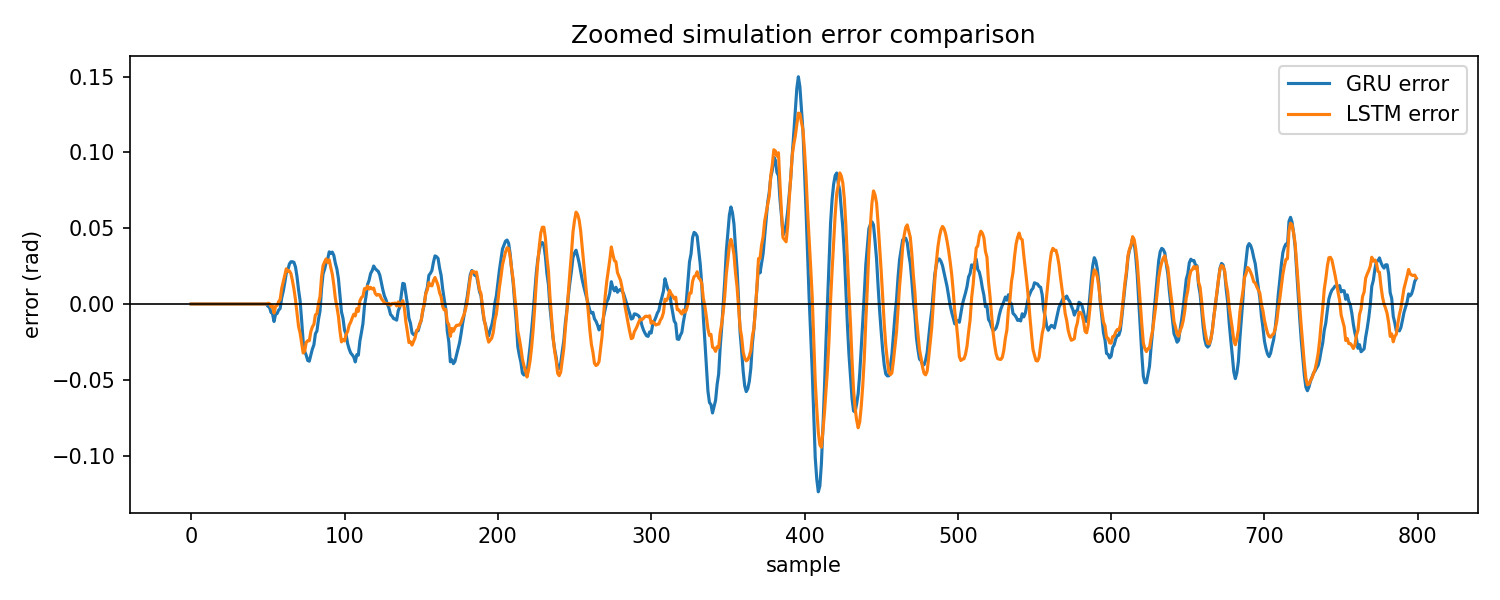
\includegraphics[width=\columnwidth]{figures/ann_simulation_error_zoom.png}}
\caption{Simulation error for the GRU and LSTM models.}
\label{fig:ann_simulation}
\end{figure}

\subsection{ANN Discussion}

The GRU was added to check whether the extra LSTM complexity was needed.
GRU is slightly better for prediction, but LSTM is better for simulation.
The main limitations are the small hyperparameter search, error
accumulation in simulation, and the fact that the ANN gives point
predictions without uncertainty estimates.
